% Created 2021-09-11 Sat 16:39
% Intended LaTeX compiler: xelatex
\documentclass[letterpaper]{article}
\usepackage{graphicx}
\usepackage{grffile}
\usepackage{longtable}
\usepackage{wrapfig}
\usepackage{rotating}
\usepackage[normalem]{ulem}
\usepackage{amsmath}
\usepackage{textcomp}
\usepackage{amssymb}
\usepackage{capt-of}
\usepackage{hyperref}
\usepackage[margin=1in]{geometry}
\usepackage{fontspec}
\usepackage{indentfirst}
\setmainfont[ItalicFont = LiberationSans-Italic, BoldFont = LiberationSans-Bold, BoldItalicFont = LiberationSans-BoldItalic]{LiberationSans}
\newfontfamily\NHLight[ItalicFont = LiberationSansNarrow-Italic, BoldFont       = LiberationSansNarrow-Bold, BoldItalicFont = LiberationSansNarrow-BoldItalic]{LiberationSansNarrow}
\newcommand\textrmlf[1]{{\NHLight#1}}
\newcommand\textitlf[1]{{\NHLight\itshape#1}}
\let\textbflf\textrm
\newcommand\textulf[1]{{\NHLight\bfseries#1}}
\newcommand\textuitlf[1]{{\NHLight\bfseries\itshape#1}}
\usepackage{fancyhdr}
\pagestyle{fancy}
\usepackage{titlesec}
\usepackage{titling}
\makeatletter
\lhead{\textbf{\@title}}
\makeatother
\rhead{\textrmlf{Compiled} \today}
\lfoot{\theauthor\ \textbullet \ \textbf{2021-2022}}
\cfoot{}
\rfoot{\textrmlf{Page} \thepage}
\titleformat{\section} {\Large} {\textrmlf{\thesection} {|}} {0.3em} {\textbf}
\titleformat{\subsection} {\large} {\textrmlf{\thesubsection} {|}} {0.2em} {\textbf}
\titleformat{\subsubsection} {\large} {\textrmlf{\thesubsubsection} {|}} {0.1em} {\textbf}
\setlength{\parskip}{0.45em}
\renewcommand\maketitle{}
\author{Houjun Liu}
\date{\today}
\title{Trauttmann}
\hypersetup{
 pdfauthor={Houjun Liu},
 pdftitle={Trauttmann},
 pdfkeywords={},
 pdfsubject={},
 pdfcreator={Emacs 27.2 (Org mode 9.4.4)}, 
 pdflang={English}}
\begin{document}

\maketitle


\section{Trauttmann}
\label{sec:orgffcc347}
\begin{itemize}
\item India affected by the successful expansion of Islam

\begin{itemize}
\item Created globalized multiculturalism
\item Expanded Indian ideas and invention to Europe

\begin{itemize}
\item Chess
\item Folktale collection
\item \emph{Panchatantra} animal fables
\item Literally Zero
\item And, Arabic Numerals (\#what)
\end{itemize}
\end{itemize}

\item Europeans interact with India

\begin{itemize}
\item Indian very strange for Europeans
\item Created legacies and mysteries about India
\item CLAIM: Images/representations were dreamlike

\begin{itemize}
\item Misrepresentation goes back to greco-Roman times
\item Viewed India as a land of strange people + desirable luxuries
\end{itemize}

\item Originally leveraged the Muslims as the point of trade, but later
developed desire to handle trade w/ India independently

\begin{itemize}
\item One attempt to do that failed very badly, i.e. Colombus. We all
know where he ended up.
\item India was thought as sprawled throughout Asia, as in\ldots{}
\end{itemize}
\end{itemize}
\end{itemize}

\begin{figure}[htbp]
\centering
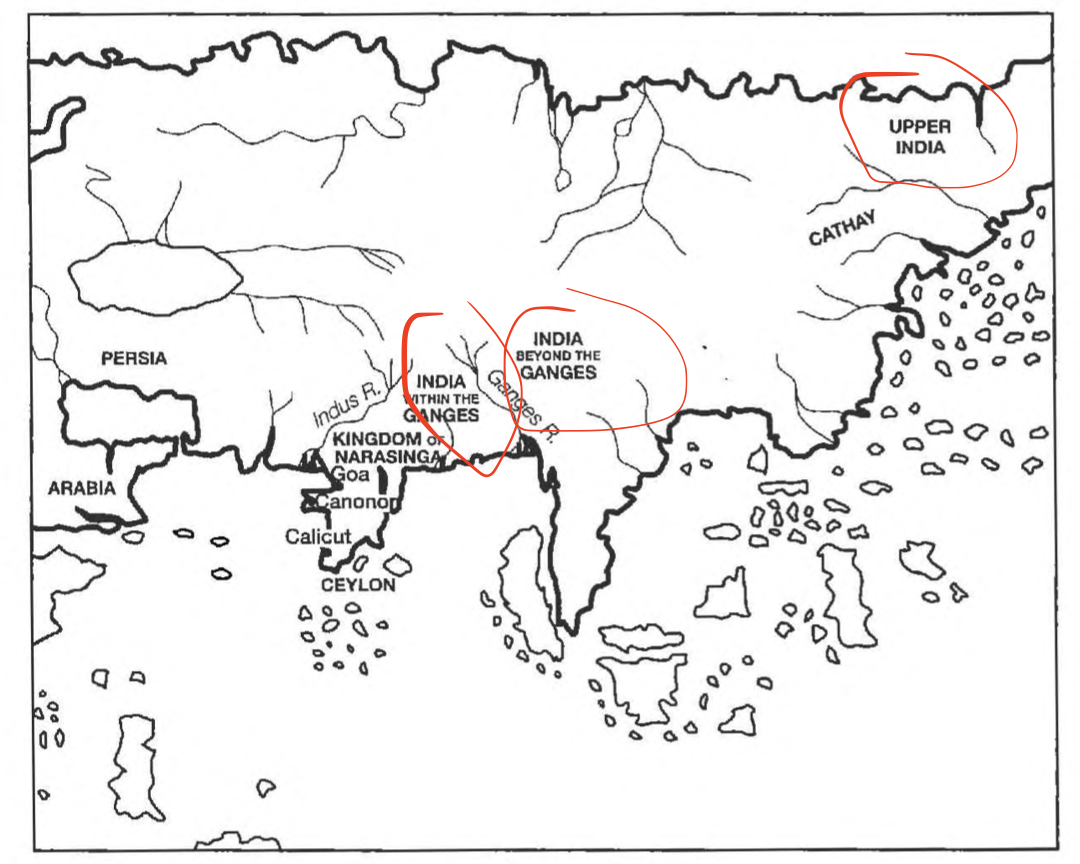
\includegraphics[width=.9\linewidth]{indiaiseverywhere.png}
\caption{indiaiseverywhere.png}
\end{figure}

\begin{itemize}
\item Portugal in India

\begin{itemize}
\item Created the first effective voyages in the Indian direction
\item Traveled around Africa to reach the coast of India, dominating
Euro-asian trade
\item Created treaties with local governments
\item Established seaborne trade domination by requiring trading licenses
\item Supplied local governments with resources

\begin{itemize}
\item American crops: potatos and corn
\item Luxuries: tobacco and pineapple
\item Other foods: tomatos and chilli
\end{itemize}

\item Also, brought Catholic Christanity with them; who could have
guessed?

\begin{itemize}
\item Converted Indians
\item Established Roman Pope's supermicy over already Existant Thomas
Christians
\item Employed two strategies

\begin{itemize}
\item Please the Indians: adopted the form of a brahmin renouncer
\item Force the Indians: instituted Inquisition to force orthodoxy
\end{itemize}
\end{itemize}
\end{itemize}

\item Porchugual vs. Spain

\begin{itemize}
\item Squabble squabble squabble
\item Eventually the\ldots{} Pope? settled the issue: awarding Portugal every
to the east of Brazil and Spain everything to the west
\end{itemize}

\item Merchant Companies

\begin{itemize}
\item Novel trading strategies
\item Created companies with independent armies that traded
\item Promoted merchantilists monopolies on a region/a good
\item Entered into political relationships to establish power = control
\item Lead companies to rule Indian territory
\end{itemize}

\item The Brits

\begin{itemize}
\item Competition spawned from rivalry between England and France

\begin{itemize}
\item Wiping French rule in Canada
\item Amercian independence w/ assistance by france
\item Establishing Bengal terrirory in India
\end{itemize}

\item CLAIM: fighting, and winning BEI.C vs. FEI.C established Britian's
Empire in India
\item Fought and implicated Indian allies

\begin{itemize}
\item Indian princes leased independently-governed trading posts
("factories") to help either one side or the other
\item Eventually BEI.C army defeated Mughal army in 1757, and
effectively achieved independence in Bengal by installing a new
governor
\item Delhi Emperor allowed BEI.C to be the political and millitary
admin (\emph{diwani}) of the region
\end{itemize}

\item Goals of doing this

\begin{itemize}
\item Failed with trading with the Dutch example
\item Struggles with the French to acquire new territory
\item Turns BEI.C from small company to one with huge rule and control
\item Company rule lasted from 1765-1858 when India is officially ruled
by the crown
\end{itemize}

\item Ruling strategy

\begin{itemize}
\item Not army based, and instead evolved from trading companies
\item Goal of rulers is to eventually retire to England + consider
Britain their home
\item Resisted the idea of colonization, otherwise may create the
Amercia problem
\item Prevented admission of non-company Europeans, including
missionaries
\item A few thousand Europeans controlling lots more indians
\item Most Europeans born and schooled in Britain and sent as adults

\begin{itemize}
\item Working under the direction of the headquarters
\item Retained British identity and ideology
\end{itemize}

\item Controlled large Indian army

\begin{itemize}
\item CLAIM: Success was more because of Indian manpower than of
military tech
\item Men were well-drilled
\item Created new organizational structures
\item Also, allied with Indian rulers

\begin{itemize}
\item Gave independent control at the price of giving up control of
foreign affairs + men for army
\item Each region had a "resident" which informed and influenced
strategic decisions
\end{itemize}
\end{itemize}
\end{itemize}

\item 1857 Mutiny

\begin{itemize}
\item Causes

\begin{itemize}
\item The Enfield rifle cartridge wsa greased with animal fat =>
offended the Hindu + Muslim
\item Policy of "Lapse" => dissolving princely states without direct
heir
\end{itemize}

\item Felt like that the religion was under attack
\item Mutiny spread across India, but it was eventually quelled after a
year because it was not unified
\item CLAIM: this showed that the Indians were discontent with British
rule
\item Aftermath

\begin{itemize}
\item Mutineers were punished harshly
\item Mughal Empire formally abolished w/ the king exiled to Burmar
\item In Nov 1, 1858, the Queen assumed control of India => direct
parlimentary control

\begin{itemize}
\item Assured that indian religions will not be interferred with
\item Rights and territories of princely states won't either
\item Reorganized to increase Britons in the Indian army
\item Harsh feelings divided India, CLAIM: leading it to gather the
new goal of turning India into a US/Europe nation state
\end{itemize}
\end{itemize}
\end{itemize}
\end{itemize}

\item India and Europe

\begin{itemize}
\item Initially worked under a interference policy

\begin{itemize}
\item Goal was not to take over
\item All had the shared goal of making money for the Company
\item Minimal government for the goal of law-and-order
\end{itemize}

\item Jesuits spreader Christianity => Beschi very successful. BEI.C
eventually prohibited it.
\item Family and civil disputes settled based on religious court; criminal
and contract law were made uniform => law that hinged on religion
remained a problem until this day
\item Company took the stance of minimal interference in land revenue,
too!

\begin{itemize}
\item Created policy of settling revenue in obligation to \emph{zamindars}
\end{itemize}

\item CLAIM: minimal interference came under pressure during attempted
Indian reform to European values

\begin{itemize}
\item Newly settled land identity on individual cultivator
\item Government reached every cultivator directory + not through
landlords
\item New reformation movements Utilitarinasm => governmental reform,
and evangelical movement => social reform
\end{itemize}

\item This reforamtion ebbed and flowed: Britian, after 1857 rebellion,
decided that they overdid it and tuned down the reformation
\item European reform of India

\begin{itemize}
\item New family + kinship rules
\item Brought the idea of popular soverenty as a cool governmental model
\item Higher respect for learning, science, and technology => turning
India from the centre of learning to not and to respecting
learning again due to THE INDUSTRIAL REVOLUTION

\begin{itemize}
\item Textiles! (destructing handicraft along with it)
\item Railway!
\item Historiography of India!
\end{itemize}
\end{itemize}
\end{itemize}
\end{itemize}
\end{document}
